\documentclass[a4paper,11pt]{article}

\usepackage[portuguese]{babel}
\usepackage[utf8]{inputenc}
\usepackage{amsmath}
\usepackage{graphicx}
\usepackage{hyperref}
\usepackage{float}
\usepackage{subfig}
\usepackage{fixltx2e}
\usepackage[bottom]{footmisc}
\usepackage{listings}
\usepackage{xargs}                      % Use more than one optional parameter in a new commands
\usepackage[pdftex,dvipsnames]{xcolor}  % Coloured text etc.
\usepackage[colorinlistoftodos,prependcaption,textsize=tiny]{todonotes}
\newcommandx{\unsure}[2][1=]{\todo[linecolor=red,backgroundcolor=red!25,bordercolor=red,#1]{#2}}
\newcommandx{\change}[2][1=]{\todo[linecolor=blue,backgroundcolor=blue!25,bordercolor=blue,#1]{#2}}
\newcommandx{\info}[2][1=]{\todo[linecolor=OliveGreen,backgroundcolor=OliveGreen!25,bordercolor=OliveGreen,#1]{#2}}
\newcommandx{\improvement}[2][1=]{\todo[linecolor=Plum,backgroundcolor=Plum!25,bordercolor=Plum,#1]{#2}}
\newcommandx{\thiswillnotshow}[2][1=]{\todo[disable,#1]{#2}}
\usepackage[font=footnotesize]{caption}
\usepackage[hypcap]{caption}
\usepackage[top=2.5cm, bottom=2.5cm, left=2.5cm, right=2.5cm]{geometry}
\usepackage{enumerate}
%\usepackage[siunitx,american]{circuitikz}

\setcounter{tocdepth}{3}
\setcounter{secnumdepth}{4}

\numberwithin{equation}{section}
\addto\captionsportuguese{\renewcommand{\contentsname}{Índice}}

\linespread{1.3}
\usepackage{indentfirst}

\begin{document}
\begin{titlepage}
\begin{center}

\hfill \break
\hfill \break


\includegraphics[width=0.3\textwidth]{img/logo}~\\[1cm] 

\textsc{\LARGE Instituto Superior Técnico}\\[0.25cm]
\textsc{\Large Mestrado Integrado em Engenharia Electrotécnica e de Computadores}\\[1.8cm]
\textsc{\huge Electrónica de Potência}\\[0.25cm]

\vspace{6mm}

{\huge \bfseries Conversor CC/CC \\[0.7cm]}
{\bfseries Redutor, Ampliador \& Redutor-Ampliador \\[1cm]}

\begin{tabular}{ l l }
	João Bernardo Sequeira de Sá & \hspace{2mm} n.º 68254 \\
	Maria Margarida Dias dos Reis & \hspace{2mm} n.º 73099 \\
	Rafael Augusto Maleno Charrama Gonçalves & \hspace{2mm} n.º 73786 \\
	Nuno Miguel Rodrigues Machado & \hspace{2mm} n.º 74236
\end{tabular}

\vspace{7mm}

Turno de Segunda-feira das 17h00 - 20h00

\vfill

{\large Lisboa,  de Novembro de 2015} 
	
\end{center}
\end{titlepage}
	
\tableofcontents
\pagebreak

\section{Introdução}

O objetivo deste trabalho é estudar o funcionamento das três principais topologias de conversores CC/CC, sendo estas o conversor redutor, conversor ampliador e redutor-ampliador.

Este tipo de conversores pode ser visto como o equivalente em corrente continua de um transformador cuja relação de transformação é variável. Quer isto dizer que através de um conversor CC/CC é possível converter uma certa fonte de tensão continua com valor fixo para uma fonte de tensão com valor variável, fazendo-se uma elevação ou redução do valor. \cite{Rashid}

Sendo assim pode considerar-se que este trabalho está dividido em três partes sendo que em cada uma destas se estuda o funcionamento de uma topologia diferente.

A primeira topologia a considerar é o conversor redutor. O objetivo neste caso é obter-se à saída uma tensão inferior à de entrada, sendo que se pode controlar esta diferença através do fator de ciclo.

De seguida estuda-se o conversor ampliador, onde o objetivo é o contrário da anterior topologia, querendo-se obter à saída uma tensão superior à de entrada. Novamente esta relação pode ser controlada através do fator de ciclo.

Por fim tem-se o conversor redutor-ampliador, onde é possível obter na saída um valor inferior ou superior da tensão de entrada. Novamente o parâmetro de controlo aqui é o fator de ciclo, onde abaixo de um certo valor se obtém uma redução da tensão e acima uma ampliação desta. Em condições de operação semelhantes este conversor não consegue obter uma redução de tensão tão grande quanto o conversor redutor e o mesmo pode ser dito entre a ampliação e o conversor ampliador.


\section{Condução do Trabalho}

\subsection{Conversor Redutor}

\subsubsection{Carga R}

No estudo do conversor redutor começa-se por considerar uma carga resistiva pura sendo o circuito considerado apresentado na \autoref{fig:Red R}

\begin{figure}[h]
	\centering
	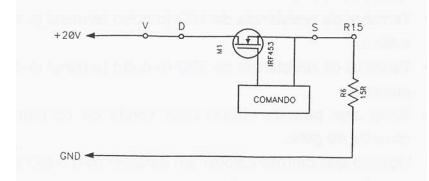
\includegraphics[keepaspectratio=true, scale=0.8]{teoricas/Redutor R.png}
	\caption{Esquema do Conversor Redutor com Carga Resistiva.}
	\label{fig:Red R}
	\vspace{-0.8em}
\end{figure}

	Após feitas as ligações necessárias, regulado o Gerador de Funções para que se obtenha o sinal quadrado com as caraterísticas desejadas.
	
\paragraph{Formas de onda da tensão V\textsubscript{GA} e corrente de \textit{Gate} para $50$ kHz}

\paragraph{Formas de onda da tensão e corrente na carga}

\subsubsection{Carga RL}

\paragraph{Formas de onda da tensão no Díodo D\textsubscript{1} e corrente na carga para $10$ kHz}

\paragraph{Frequência limiar do regime lacunar}

\subsubsection{Carga RLC}

\paragraph{Formas de onda da tensão V\textsubscript{DS} e corrente I\textsubscript{D} para $20$ kHz}

\paragraph{Formas de onda da tensão e corrente no Díodo D\textsubscript{1}}

\paragraph{Formas de onda da tensão na carga e corrente na bobine}

\paragraph{Tensão na carga em função do fator de ciclo}

\paragraph{Efeito da adição de um \textit{Snubber} entre o Dreno e \textit{Source} do MOSFET para $50$ kHz}

\paragraph{Forma de onda da tensão V\textsubscript{AK} do Díodo D\textsubscript{1} para $200$ kHz}

\subsection{Conversor Ampliador}

\paragraph{Formas de onda da tensão V\textsubscript{DS} e da corrente I\textsubscript{D} para $40$ kHz}

\paragraph{Formas de onda na Resistência e corrente em D\textsubscript{1}}

\paragraph{Tensão na carga em função do fator de ciclo}

\subsection{Converor Redutor-Ampliador}

\paragraph{Formas de onda da tensão e corrente aos terminais da bobina para $40$ kHz}

\paragraph{Formas de onda da tensão na Resistência e corrente D\textsubscript{1}}

\paragraph{Tensão na carga em função do fator de ciclo}

\paragraph{Rendimento do conversor para um fator de ciclo de $60$ \%}

\pagebreak

\begin{thebibliography}{2}
	
	\bibitem{Kassakian}
	Kassakian, John G. et al (1992, June), Principles of Power Electronics, \textit{Addison-Wesley Publishing Company}

	\bibitem{Rashid}
	Rashid, Muahammad H. (2004), Power Electronics - Circuits, Devices and Applications, \textit{Prentice Hall}
	
	\bibitem{Silva}
	Silva, Fernando (1998), Eletrónica Industrial, Fundação Calouste Gulbenkian
	
\end{thebibliography}


\pagebreak



\end{document}
